\section{Organisationsplan för hela projektet}
Beställning av projektet har gjorts av kunden, och det är kunden som levererat kravspecifikationen och på så sätt avgör om den är uppfylld eller inte. Det är även kunden som står för betalning av den slutgiltliga produkten, som i detta fall kommer vara i form av högskolepoäng. All kontakt med kunden och annan kontakt utåt ligger på projektledaren. Projektledaren ska också planera arbetet i gruppen och se till att hela gruppen arbetar mot ett och samma mål. Arbetet i sig ligger dock inte enbart på projektledarens axlar, utan även på resterande gruppmedlemmar, där alla, inklusive projektledaren, spelar lika stor roll i arbetets utförande. Det finns även en handledare tillgänglig som experthjälp för att hjälpa gruppen på vägen. Figur \ref{organisationsplan} illustrerar organisationsstrukturen.

\begin{figure}[H]
	\begin{center}
		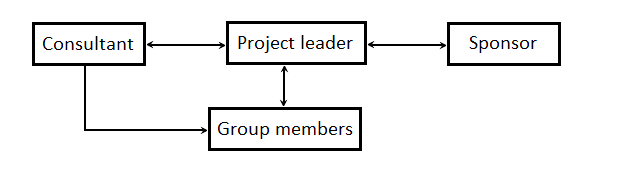
\includegraphics[keepaspectratio=true,width=375px]{grafik/organisationsplan.png}
		\caption{Organisationsplan}
		\label{organisationsplan}
	\end{center}
\end{figure}

\subsection{Villkor för samarbete inom projektgruppen}
Inom gruppen har vi kommit överens om att följande gäller:
\begin{itemize}
\item{Alla skall komma väl förberedda till möten.}
\item{Meddela i tid om man inte kan närvara vid ett möte. Vid sjukdom skall detta meddelas snarast.}
\item{Man skall delta vid möten som gruppen kommit överens om.}

\item{Om man är osäker på något ska man först söka information på egen hand eller ta upp detta med gruppen. I andra hand bör någon extern person tas kontakt med.}
\item{Om någon inte bidrar tillräckligt till projektet så har resterande gruppmedlemmar rätt att diskutera detta med handledare.}
\end{itemize}

\newpage